\documentclass[11pt,a4paper]{article}
\usepackage[utf8]{inputenc}
\usepackage[french,frenchb,francais]{babel}
\usepackage[T1]{fontenc}
\usepackage{amsmath}
\usepackage{amsfonts}
\usepackage{amssymb}
\usepackage{graphicx}
\usepackage{hyperref}
\author{\textsc{\textbf{Phélipot Pascal}}\\\textsc{Noro Geoffrey}\\\textsc{Ralijaona Tiona}\\\textsc{Rimoux Quentin}}
\title{Projet de BDD : Gestion au Moyen Age}
\date\today

\begin{document}
\maketitle
\pagestyle{plain}
\newpage\pagenumbering{Roman}
\tableofcontents

\newpage\pagenumbering{arabic}
\section{Introduction}
\subsection{L'idée}
Le projet est un jeu par navigateur orienté stratégie en multijoueur. 
Chaque joueur dispose d'une base sur une carte. Il a la possibilité d'y construire des bâtiments, de gérer ses ressources et de lancer la recherche de nouvelles technologies.
Les ressources sont générées chaque minute pour chaque utilisateur et il faut améliorer ses bâtiments pour en produire plus. \\
Le but du jeu est d'attaquer les autres joueurs afin de gagner des ressources et d'améliorer sa base au maximum. \\


\subsection{Répartition des rôles}
\subsection{Mise en œuvre}
\begin{itemize}
	\item Carte du monde 
	\item Moteur du jeu \\
	La création du moteur du jeu a été attribuée à Pascal. Il doit réaliser la gestion des tours.
	\item Affichage

	\item Données \\
	Tout le monde a participé à l'ajout de nouvelles unités et de bâtiments.
\end{itemize}
\subsection{Gestion de projet}
Pour gérer ce projet nous avons bosser tout ensemble simultanément grâce à la plate-forme Github, qui permet de gérer la version de son code et de fusionner les travaux de chacun.\\
Le projet est accessible en ligne à l'adresse :  \url{http://www.github.com/pasterp/GestionMiddleAge}

\newpage\section{Représentation des données}
\subsection{Modèle-Vue-Contrôleur}
\subsection{Encapsulation}
\subsection{Base de Données}

\newpage\section{Gestion des tours}
Pour gérer les actions des joueurs, on a besoin de la notion du temps. Il faut donc que notre site opère certaines opérations au fil du temps. \\
Il va devoir attendre une certaine durée (qu'on appellera cycle) qui a été définie à 15 minutes et ensuite lancer des actions telles que la génération des ressources, l'avancée d'une armée, etc...\\
\subsection{Les possibilités}
\subsubsection{Ajax}
L'AJAX (Asynchronous JavaScript and XML) est un outil permettant via un Javascript de modifier la structure d'une page en direct. 
Ce dernier peut donc appeler les fonctions désirées quand un utilisateur est présent sur une page.\\
L'avantage de cette méthode est qu'elle est transparente à l'utilisateur et qu'elle permet de faire des modifications dynamiques sur la page qu'il a devant lui. \\
L'inconvénient est qu'il est nécessaire d'inclure un fichier supplémentaire et que les appels seront très concentrés sur le serveur lors de l'utilisation par un grand nombre d'utilisateur.\\
\subsubsection{Tache cron}
La tâche Cron est un système au niveau système qui permet de lancer un script à des dates et heures précises. Néanmoins Cette fonctionnalité demande des droits spécifiques au système et ne peut donc être mise en oeuvre à l'IUT. Cette méthode aurait perdu de faire un appel minimum aux fonctions (juste aux horaires désirés);
\subsection{Mise en œuvre}
La solution retenue est hybride : elle est codée en PHP mais est appelée par l'utilisateur. \\
Chaque page chargée entraine une vérification de l'heure du dernier cycle, PHP compare ensuite si ce cycle est assez ancien pour faire un nouveau cycle (900 secondes dans notre code) et si c'est le cas il lance les fonctions de génération de ressources.

\newpage\section{Possibilités d'améliorations}

\newpage\section{Conclusion}
\subsection{Avis personnels}
\subsubsection{Noro Geoffrey}
\subsubsection{Phélipot Pascal}

\subsubsection{Ralijaona Tiona}
\subsubsection{Rimoux Quentin}
\subsection{Avis Global}

\newpage\pagenumbering{Roman}
\section{Annexes}
\subsection{Base de données}
\begin{figure}[!h]
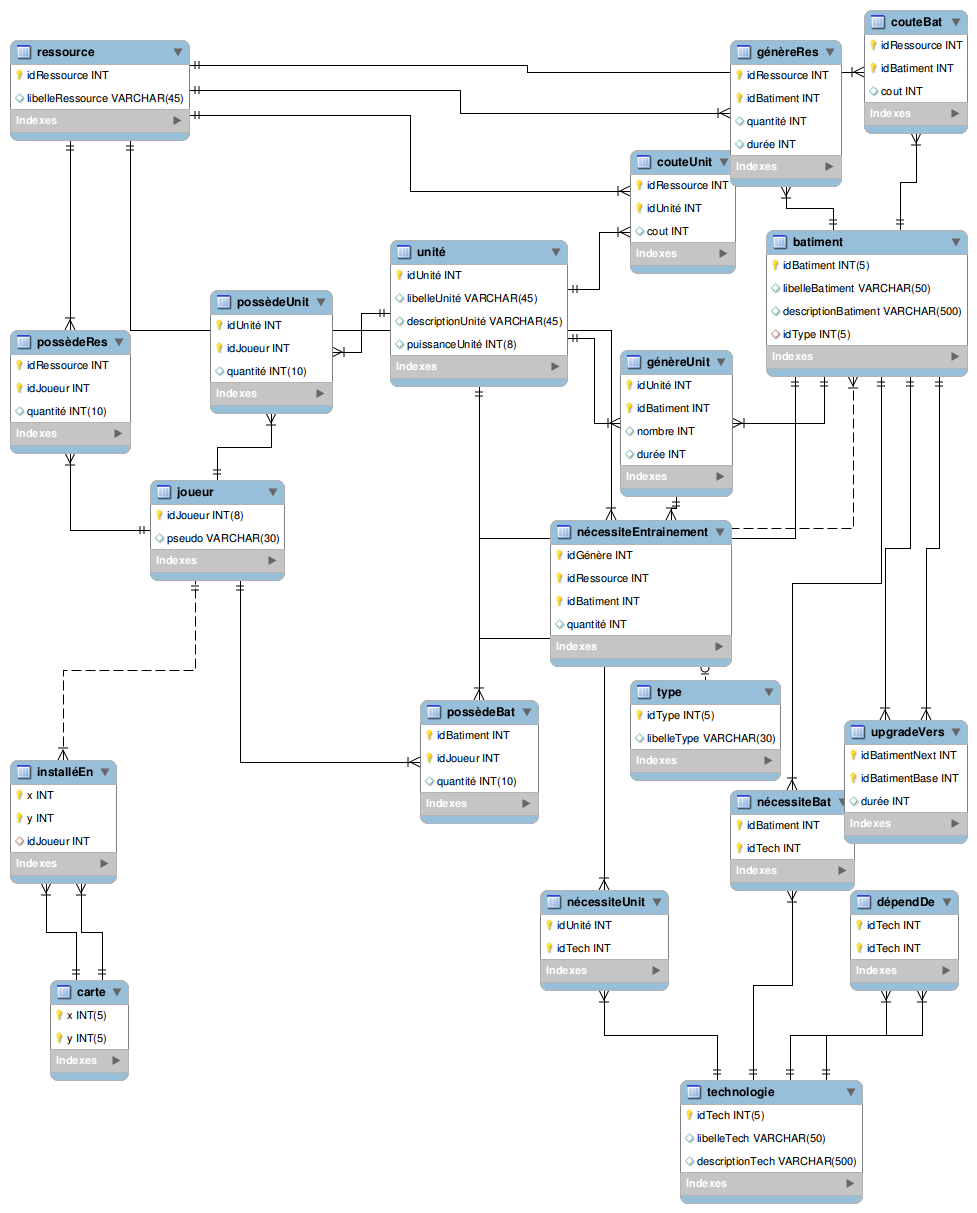
\includegraphics[scale=0.3]{./sql/last.png}
\end{figure}
\end{document}